%storm
\documentclass[../../main/main.tex]{subfiles}


\begin{document}
\title{Background}


%%%%%%%%%%%%%%%%%%%%% Chapter STORM %%%%%%%%%%%%%%%
\chapter{Background And Introduction to STORM}\label{chp:storm}
This chapter provides an introduction to \glsentrylong{storm} (\glsentryshort{storm}).  \gls{storm} falls within the field of \glsentrylong{se} (\gls{se}) and the sub-discipline of \glsentrylong{sse} (\gls{sse}). To familiarize (or refresh) the reader, this chapter begins with some background on \gls{se} and \gls{sse}.  The \gls{se} concept of system life-cycle phases and the \gls{sse} Framework are introduced.  Following this, \gls{storm} and it's components (\gls{stpasec} and \gls{csbd}) are introduced.  The chapter concludes with a discussion of the patrol base operations as a sample systems to which  \gls{storm} is applied.

%%%%%%%%%%%%%%%%%%%%% Section SE %%%%%%%%%%%%%%%
\section{Systems Engineering}\label{sec:stormse}
\begin{quote}
\textit{"Systems Engineering is an interdisciplinary approach and means to enable the realization of successful systems. It focuses on defining customer needs and required functionality early in the development cycle, documenting requirements, then proceeding with design synthesis and system validation while considering the complete problem..."
}\end{quote}
\begin{flushright} International Council on Systems Engineering \end{flushright} 

A system is a set of interacting and interdependent components that act as a whole,  through various mechanisms, to perform some function. Systems engineering is a multidisciplinary approach to solving problems related to large and complex man-made systems.  It focuses on stakeholder needs and assets while minimizing asset losses.  It focuses on building the right product.  It avoids building the wrong product or building the right product incorrectly.  

According to Holstein and Bode's, who summarized systems engineering for the Encyclopedia Britannica, systems engineering probably developed from the overlapping of engineering concepts from different fields. They note that, for example, both chemical and mechanical engineering focus on heat transfer, and cybernetics and computer theory are both sub-disciplines of electrical and electronics engineering.   But, at its core is the scientific methodology and the use of mathematical modeling.  Holstein and Bode link the more recent emergence of systems engineering to the communications industry (telephony, in particular) and Britain's post-World War II operations research.

The emergence of systems engineering and its growing popularity is linked to the growing complexity of systems.  Systems are composed more and more of numerous interacting parts.  These interacting parts often exhibit emergent properties.  These are properties that arise from the interactions of many components.  These properties are not attributable to any one component and thus require a systems-thinking perspective. Holstein and Bode site the Nike Ajax U.S. Air Defense System as one of the earlier examples of these system-level emergent properties. Tactical range of the Ajax requires consideration of multiple factors including aerodynamic design, maneuverability provided by the control systems, warhead size and weight, etc.  Other factors include feedback from radar and the autopilot.  Achieving tactical range emerges from analysis of the many interacting components.  

\Glsentrylong{se} is often employed in the communications and computing industries. But, it works in any field that works with large complex systems.  The applicability of systems engineering to other fields is promoted, in part, by the increased capacity to manage complex systems that arise from the increased computational power available.  Computational power and thus complexity will only grow in the future, and consequently, so will the need for competent systems engineers.

The relevant \glsentryshort{se} standards are defined in ISO/IEC/IEEE\footnote{ISO = \glsentrylong{iso}; IEC = \glsentrylong{iec}; and IEEE = \glsentrylong{ieee}} 24748-5 \cite{iso247482017} and ISO/IEC/IEEE 25288\footnote{These standards reference other relevant standards.} \cite{iso15288}.  These standards define the concept of system life-cycle phases: concept, development, production, utilization, support, and retirement.  The concept and development phases are the focus of \gls{storm} because safety and security should be considered during the design phase.  However, the support phase is also relevant for re-envisioning and updating the system.  

%%%%%%%%%%%%%%%%%%%%% Section SSE %%%%%%%%%%%%%%%
\section{Systems Security Engineering}\label{sesc:sse}
\begin{quote}
\textit{"The ultimate objective is to obtain trustworthy secure systems that are fully capable of supporting critical missions and business operations while protecting stakeholder assets, and to do so with a level of assurance that is consistent with the risk tolerance of those stakeholders."}
\end{quote}
\begin{flushright} Ron Ross (\gls{nist}) (Quoted from NIST SP 800-160 \cite{NIST800160}) \end{flushright} 

Systems Security Engineering (\gls{sse}) is a sub-discipline of Systems Engineering (SE).  It applies scientific, mathematical, and related technical concepts and procedures to engineer trustworthy systems that meet stakeholder needs. 

Systems Security Engineering probably developed alongside systems engineering.  But, the need for security engineering is becoming more and more on the forefront of everyone's minds in today's technology-dependent society.  With recent high-profile security breaches such as the Target  security leak (\$18.5 million legal settlement \cite{target}) and the disastrous Snowden leaks (cost of leak unknown), companies can no longer afford to take a relaxed posture on security.  This need for security is stated no better than by experts in the field

\begin{quote}
\textit{"With the continuing frequency, intensity, and adverse consequences of cyber-attacks, disruptions, hazards, and other threats to federal, state, and local governments, the military, businesses, and the critical infrastructure, the need for trustworthy secure systems has never been more important to the long-term economic and national security interests of the United States. Engineering-based solutions are essential to managing the growing complexity, dynamically, and interconnectedness of today's systems, as exemplified by cyber-physical systems and systems-of-systems, including the Internet of Things."}  \cite{NIST800160}
\end{quote} \begin{flushright}\gls{nist} Special Publication 800-160 vol 1 \cite{NIST800160}.\end{flushright}


Systems Security Engineering is applied whenever security is a component of systems engineering.  As a multi-disciplinary, subspecialty of systems engineering, \gls{sse} focuses on stakeholder assets and loss avoidance or mitigation.  The Systems Security Engineering Framework defines the context in which \gls{storm} applies.
   
%%%%%%%%%%%% Systems Security Engineering Framework %%%%%%%%%%%%%%
\subsection{Systems Security Engineering Framework}
The authoritative document on \gls{sse} is the \gls{nist} Special Publication 800-160 Volumes 1 and 2.  In particular, volume 1 defines the \gls{sse} Framework.  This framework defines \gls{sse} activities that ensure the stakeholder's definition of security and asset valuation informs the system's security design.  A diagram of the framework is shown in figure \ref{sseframework}.

\begin{figure}[h]
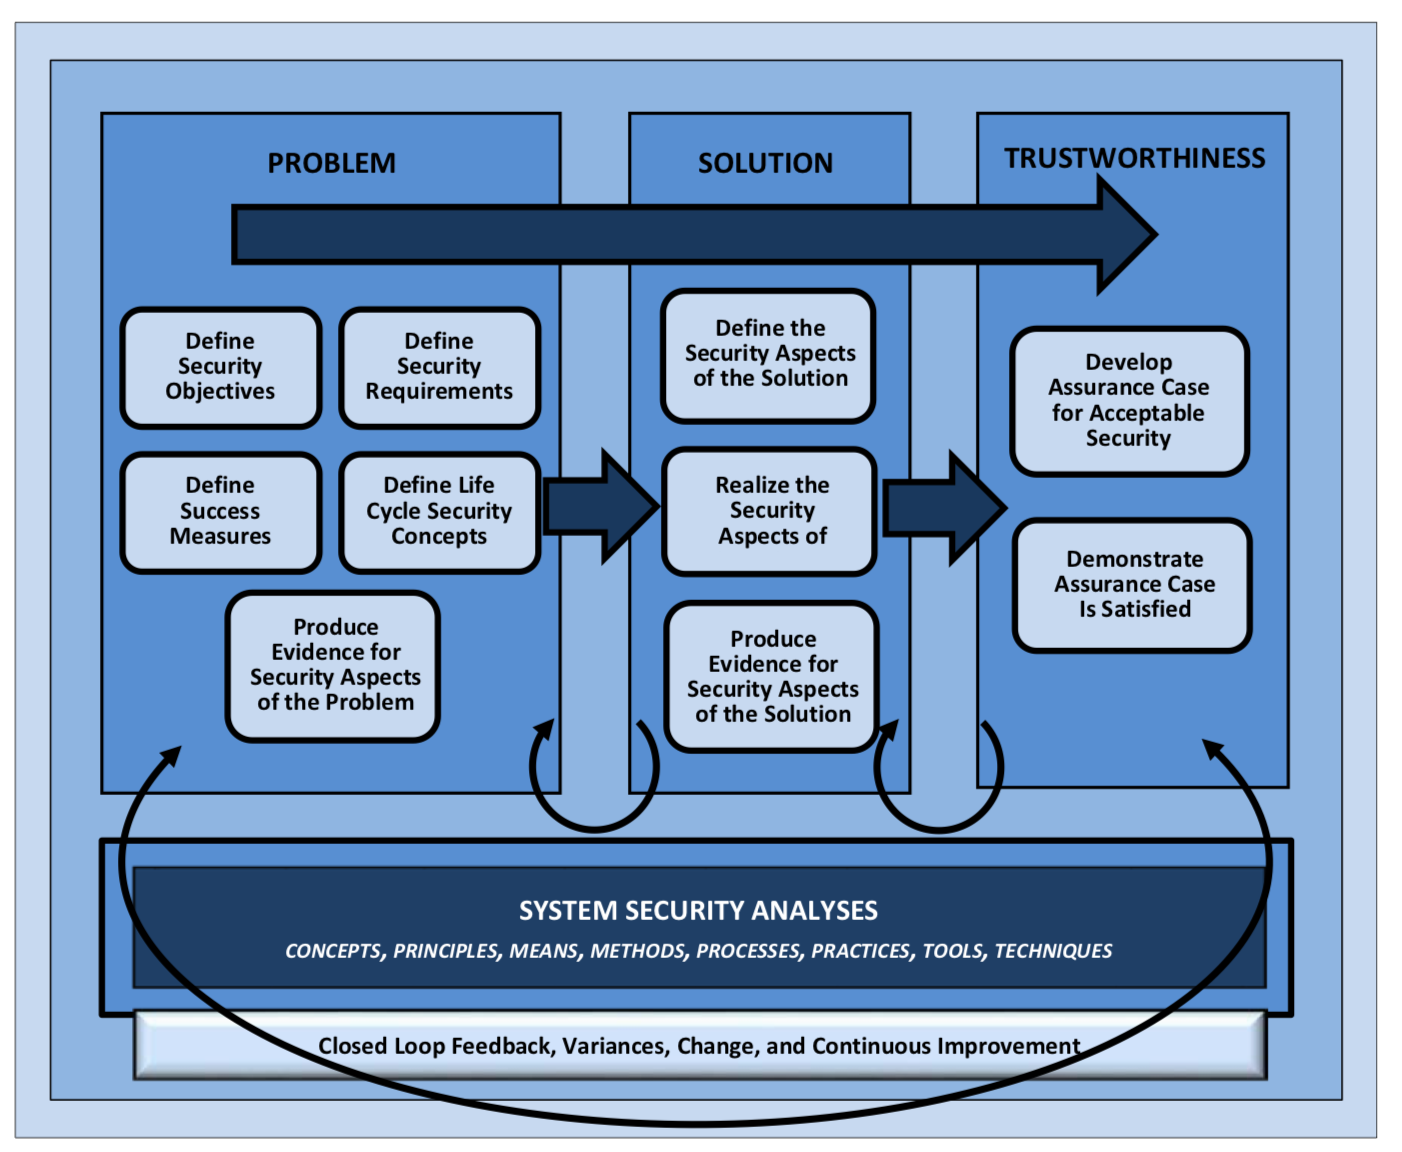
\includegraphics[width=\linewidth]{../figures/sseframework}
\caption{\label{sseframework}Systems security engineering Framework. (Image from \gls{nist} Special Publication 800-160 Vol 1: Systems Security Engineering Considerations for a Multidisciplinary Approach in the Engineering of Trustworthy Secure Systems.\cite{NIST800160})}
\end{figure}

The framework describes the problem, solution, and trustworthiness activity contexts.  These three contexts are further refined. 
\paragraph*{Problem}
The problem phase focuses on defining security from the stakeholder's needs, purpose, and mission.  It is divided into four sub-contexts (activities).  The first activity defines the security objective. What does it mean to be "\textit{adequately secure}"?   What are the assets and asset losses?  Which losses are unacceptable?
 
The second activity defines measures of success.  What level of asset protection is required?  What level of assurance or protection is required?  

The third activity defines the system life-cycle security concepts.  What is the system security context throughout the life-cycle of the system?  What processes, methods, and procedures throughout the system's life cycle need security?  

The fourth activity defines the security requirements.  The stakeholder security requirements are determined from the previous three activities.

\paragraph*{Solution}
With the problem defined, the solution activity transforms the problem into security design requirements.  This has three activities.  The first activity defines the security aspects of the solution. Six aspects are listed in \gls{nist} SP 800-160: protection strategy; security design requirements; security architecture view and viewpoints; security design; security procedural aspects, capabilities, and limitations in the system life-cycle; and how to verify and measure security performance. 

The next activity realizes the security aspects.  This is the security implementation phase.

The last activity produces evidence for the security aspects of the solution. This can be obtained from a variety of \gls{sse} verification methods.  This evidence is compared with claims measured against the stakeholder's requirements.

\paragraph*{Trustworthiness}
Once the solution is generated, the trustworthiness context develops assurance cases and demonstrates that they are satisfied.  The first activity develops and maintains assurance cases for acceptable security.  \gls{nist} SP 800-160 defines assurance case as \textit{"a well-defined and structured set of arguments and a body of evidence showing that a system satisfies specific claims with respect to a given quality attribute."}  Assurance cases also provide auditable artifacts supporting the system security claims.

The second trustworthiness activity demonstrates that the assurance case is satisfied.  A subject-matter expert should evaluate the assurance case to determine if the evidence supports the security claims.

\subsubsection{Conforming to The SSE Framework}
\gls{storm}is consistent with the \gls{sse} Framework.  It is up to the \gls{storm} user to verify in detail that \textit{all} nine sub-contexts of the \gls{sse} Framework are addressed.  

\gls{storm}'s two components in combination satisfy all three \gls{sse} Framework contexts.  The problem and solution contexts are covered by \gls{stpa}/\gls{stpasec}.  The trustworthy context is covered by \gls{csbd}.  Both \gls{stpa}/\gls{stpasec} and \gls{csbd} are described in the following sections.


%%%%%%%%%%%%%%%%%%%%% Section STORM %%%%%%%%%%%%%%%
\section{STORM}\label{sec:storm}

\glsentrylong{storm} (\gls{storm}) is an approach to managing risk and engineering trustworthy systems that satisfy stakeholder requirements and conform to industry standards.  It applies state-of-the-field analysis techniques to design products that are safe, secure, and integral.  It applies formal methods to produce reproducible and auditable verification demonstrating that stakeholder claims are satisfied.  


\gls{storm} is a new approach to implementing the Systems Security Engineering Framework.  It can also be used in conformance to the \gls{iso}/\gls{iec}/\gls{ieee} 15288 and 24748 standards.  

\gls{storm} is the result of the collaborative effort of Professor Shiu-Kai Chin of the College of Engineering and Computer Science at Syracuse University, Erich Devendorf, PhD of the U.S. Air Force Research Laboratory, and William Young, PhD of the U.S. Air Force 53rd Electronic Warfare Group.  

\gls{stpa} is the culmination of years of research in safety engineering by \Gls{mit} professor Nancy Leveson.  Whereas \gls{stpa} focuses on safety engineering, \gls{stpasec} focuses on security engineering.  \gls{stpasec} is the work of Dr. Young, who presented it as his PhD thesis in 2014 at \gls{mit}.  

\gls{csbd} is derived from the work of Professor Shiu-kai Chin and Professor Susan Older (also of the College of Engineering and Computer Science at Syracuse University).  They wrote the text on \textit{Access Control, Security, and Trust: A Logical Approach} \cite{ChinOlder} from which \gls{csbd} is derived.  Professor Shiu-Kai Chin teaches components of \gls{csbd} at Syracuse University in the College of Engineering and Computer Science.  


All elements of \gls{storm} are currently employed by the U.S. Air Force. \gls{stpasec} is part of the U.S. Air Force doctrine. Components of \gls{storm} are taught at Syracuse University, in particular \gls{csbd}. \gls{csbd} has also been used in the design of JP Morgan Company's SWIFT protocols \cite{pkm} and the F-16 Viper payload controller and secure memory loader verifier (not published). As this master thesis is being written, \gls{storm} is being presented to the \gls{nsa} to strengthen their mission assurance objectives.


%%%%%%%%%%%%%%%%%%%%% Subsection STORM %%%%%%%%%%%%%%%
\subsection{STAMP}\label{ssec:stamp}
\glsentrylong{stamp} (\gls{storm}) is the model that underlies \gls{stpa}, which underlies \gls{stpasec}.  Figure \ref{stampstpa} shows the relationship between \gls{stpasec}, \gls{stpa}, and \gls{stamp}.


\gls{stamp} is a way of thinking about how accidents occur.  It assumes both a traditional and a system-theoretic view.  In the traditional view, accidents are caused by unsafe chains of events.  In the system theoretic view, accidents are also caused by dynamic and complex interactions. 


\begin{figure}[h!]
\centering
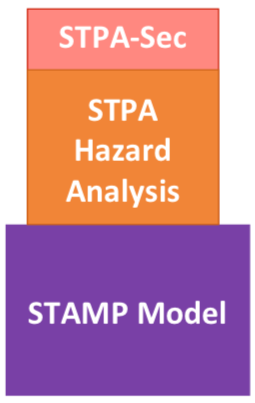
\includegraphics[width=0.3\linewidth]{../figures/stampstpa}
\caption{\label{stampstpa}Relationship between \gls{stpasec}, \gls{stpa}, and \gls{stamp}. (Image from Dr. William Young and Reed Prada 2017 \gls{stamp} Conference presentation in Boston, MA on March 27, 2017 \cite{youngPorada})}
\end{figure}

\gls{stamp} is the subject of yearly conferences world wide promoted by the Partnership for Systems Approaches to Safety and Security (PSASS)\footnote{See \url{https://psas.scripts.mit.edu/home/other-stamp-meetings/}.}.  When compared to other accident models, \gls{stamp} is more effective.\footnote{See, for example, Paul Stukus' thesis dissertation on how \gls{stamp} outdid other techniques when analyzing a U.S. Coast Guard Buoy Tender Integrated Control System \cite{buoy}} It also cost less to implement \cite{stpa}.

The need for a new hazard analysis paradigm arises near the turn of the century from the culmination of years of research into safety engineering by \gls{mit} professor Nancy Leveson.  This research reveals a need for new tools in safety analysis.  Current tools, at one time effective, are proving ineffective in managing the complexities associated with technologies of the modern era.  The current practice of analyzing individual component reliability and chain-of-causality failures does not capture the hazards associated with today's complex systems.  These systems require a system-theoretic approach to hazard analysis. 

System theory focuses on the system as a whole rather than as a collection of subcomponents.  The need for a system theory approach is epitomized in the notion that the whole is greater than the sum of its parts.  From the complex interactions of individual components arise emergent properties. These properties can be thought of as a higher order that is not predictable from the behavior of the individual components.

\gls{stamp} forms the foundation of the new, modern era systems-theoretic safety analysis techniques.  Several approaches to safety engineering are built upon the \gls{stamp} foundation.  \glsentrylong{stpa} (\gls{stpa}) is one these analysis techniques.  In addition to \gls{stpa} (the topic of the next section), several other analysis techniques are built on top of the \gls{stamp} foundation.  These include \gls{cast}, \gls{stpa} for security (\gls{stpasec}), \gls{stpa} for privacy (STPA-Priv), STPA-SafeSec \cite{safe}, and SAFE (a refinement focused on hardware and software subsystems \cite{safe}).

 At \gls{stamp}'s core is a top-down model that views accidents as dynamic control problems.  It focuses on safety constraints, hierarchical control structures, and process models \cite{saferworld}. 

\paragraph*{safety constraints}
\gls{stamp} views constraints, rather than events, as the safety-critical processes.  A lack of constraints can lead to a hazardous system state which will lead to an accident in the worst-case scenario.  

There are two types of constraints (or controls), passive and active.  Passive controls prevent unsafe conditions by their presence.  For example, lead shielding surrounding radioactive material minimizes radioactive exposure merely by its presence.  

Active controls, on the other hand, are more complicated.  They require some form of interaction to prevent unsafe conditions.  For example, a Geiger counter signaling a computer that radioactive levels are unsafe minimizes exposure by sounding an alarm which causes personnel to evacuate.  

\paragraph*{hierarchical control structures}
Figure \ref{controlmodel} is an example of a hierarchical control model.  The flow of control is from top to bottom; higher-level control structures control lower-level control structures. Downward pointing arrows indicate instructions to lower level controllers or controlled processes.  Upward pointing arrows indicate feedback from lower components.   

\begin{figure}[h!]
\centering
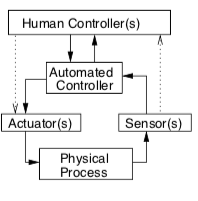
\includegraphics[width=0.5\linewidth]{../figures/controlmodel}
\caption{\label{controlmodel} Example of a control model. (Image captured from the \gls{stpa} Handbook \cite{stpa}.)}
\end{figure}
The cause of accidents is inadequate control at higher levels, which trickle down to lower levels causing hazardous conditions.  

\gls{stamp} considers four types of inadequate control on constraints: insufficient or missing constraints, wrong constraints, out-of-order or under-timed constraints, and constraints that are imposed for too long. 

\paragraph*{process models}
Figure \ref{processmodel} shows a controller with a process model.  Each controller has its own process model.  The process model describes the controller's understanding of how the system works as well as knowledge about the state of the system.  

If the controller's process model is somehow flawed or not consistent with the system's state, it could cause a hazardous condition which could cause unacceptable losses in the worst-case scenario.

\begin{figure}[h!]
\centering
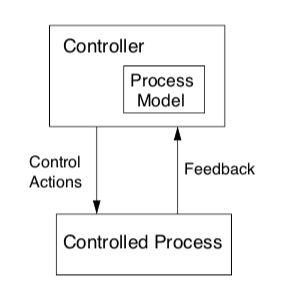
\includegraphics[width=0.5\linewidth]{../figures/processmodel}
\caption{\label{processmodel} Controller with process model. (Image captured from the \textit{Engineering a Safer World} Handbook \cite{saferworld}.)}
\end{figure}
%%%%%%%%%%%%%%%%%%%%% Subsection STORM %%%%%%%%%%%%%%%
\subsection{STPA/STPA-Sec}\label{ssec:stpa}
System-Theoretic Process Analysis (STPA) is a systems engineering methodology that helps the engineer identify and mitigate stakeholder losses. It does this using a four step process that is founded on the System-Theoretic Accident Model and Processes (STAMP).  Whereas STAMP is a way of thinking about the causes of accidents, \gls{stpa} is a method to analyze systems in order to prevent or mitigate losses caused by these accidents.  

\gls{stpa} follows the guidelines described in \gls{iso}/\gls{iec}/\gls{ieee} 15288 for System Life-Cycle Processes.  It's focus is on the Technical Processes (gls{iso}/\gls{iec}/\gls{ieee} 15288), the concept and development stage of the system life cycle (defined in ISO/IEC/IEEE 24748), and the problem and solution contexts of the Systems Security Engineering Framework (\gls{nist} SP 800-160).

\gls{stpa}, like \gls{stamp}, is the work of Professor Nancy Leveson from \gls{mit}.  \gls{stpasec} is William Young's (PhD and Col. in USAF) PhD thesis dissertation.  It is a modification of \gls{stpa} that adds on a security component.  

In a 2013 paper, Professor Nancy Leveson and Dr. William Young define safety and security as
\begin{description}
\item[ Safety ] protecting a system against \textit{unintentional} disruptions.
\item[ Security ] protecting a system against \textit{intentional} disruptions.
\end{description}
The primary difference between \gls{stpa} and \gls{stpasec} is that \gls{stpa} thinks about how \textit{accidents} arise from system-level \textit{hazards} whereas \gls{stpasec} thinks about how \textit{losses} arise from system-level \textit{vulnerabilities}.  Application of the four steps is similar for both \gls{stpa} and \gls{stpasec}.


\section{STPA/STPA-Sec Overview: Four Steps}
\gls{stpa} is a four step process.  Figure \ref{4step} diagrams these four steps.  The four steps are briefly described below.  They are applied to the patrol base operations in the next chapter. 


\begin{figure}[h]
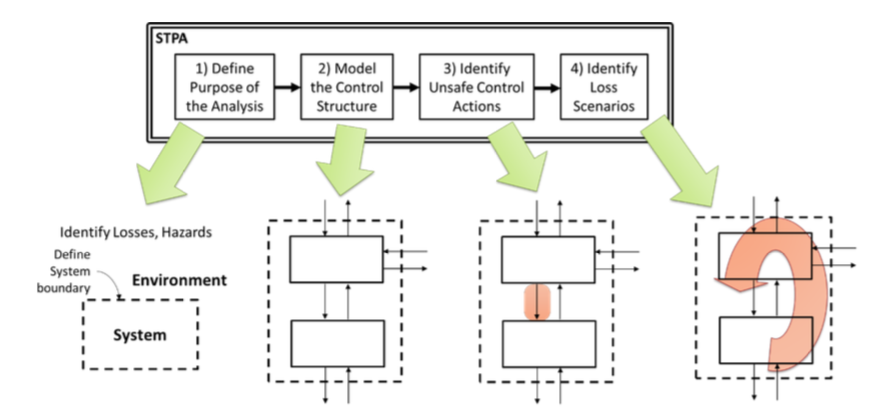
\includegraphics[width=\linewidth]{../figures/4step}
\caption{\label{4step} Four step process of \gls{stpa}. (Image captured from the \gls{stpa} Handbook \cite{stpa}.))}
\end{figure}

\paragraph*{Step 1: Define The Purpose of The Analysis}
The first step defines the purpose of the analysis and the system to be produced.  Unacceptable losses/accidents are defined by the stakeholders.  Then, system-level vulnerabilities/hazards are defined and linked to the losses/accidents they would cause in the worse-case scenario.  Next, system-level constraints are defined and linked to vulnerabilities/hazards. 

\paragraph*{Step 2: Model The Control Structure}
The second step models the system's functional control structure.  This describes the flow of control (or information) in the system.  Figure \ref{controlmodel} shows an a generalized control structure.  

The control structure shines light on system-level hazards.  Figure \ref{stpasecControlStructure} shows a control structure with the potential vulnerabilities/hazards labeled.
\begin{figure}[h]
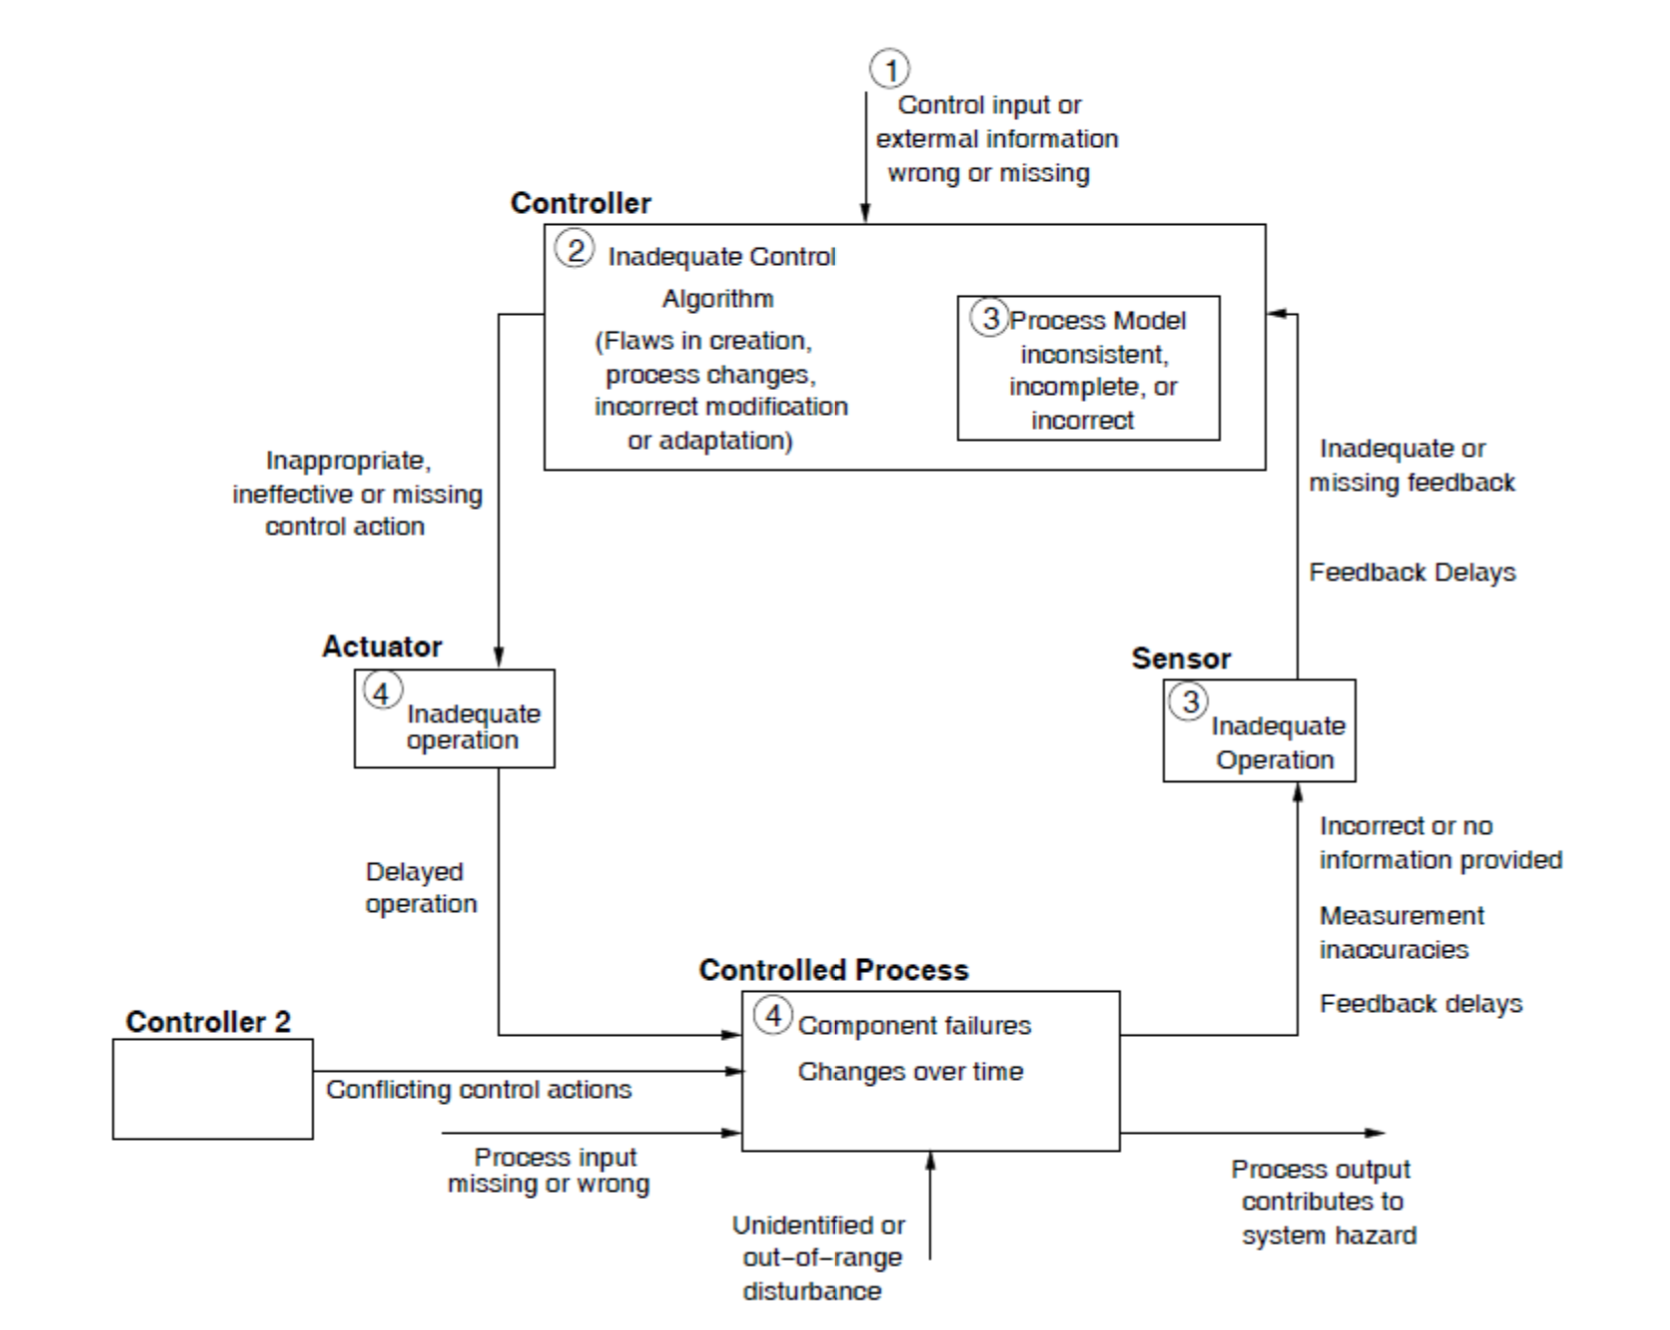
\includegraphics[width=\linewidth]{../figures/stpasecControlStructure}
\caption{\label{stpasecControlStructure} Control structure with potential system-level vulnerabilities/hazards and security considerations. (Image captured from  \textit{Systems thinking for safety and security} \cite{sys4sec}.)}
\end{figure}

(1) and (3) type vulnerabilities/hazards are caused by representation flaws.  These include missing or incorrect information or feedback and flaws involving the controller's model of the system.  (2) type vulnerabilities/hazards are caused by algorithm flaws (algorithms implement the controller's process model).  (4) type vulnerabilities/hazards are caused by component failures.

The control structure consists of two controllers, one at the top and one near the bottom and to the left.  The lower control structure could represent an adversary sending conflicting instructions to the controlled process (bottom of diagram).  

\paragraph*{Step 3: Identify Unsafe Control Actions}
The next step identifies \gls{uca} for each control action described in step 2. Control actions are instructions (commands, etc.) output by one control structure and input to another, typically from a higher to a lower control structure.   There are four types of \gls{uca}s.

\begin{itemize}
\item Not applying the control action
\item Applying the wrong control action
\item Applying the control action in the wrong order
\item Applying the control action for two long or not long enough.
\end{itemize}

In this step, each control action is analyzed for all four types of \gls{uca}s to check for vulnerabilities/hazards.  \gls{uca}s are further analyzed in step 4.


\paragraph*{Step 4: Identify Loss Scenarios}
The last step identifies scenarios that could cause the \gls{uca}s discovered in step 3.  Each scenario describes how a \gls{uca} could cause a system-level vulnerability/loss in the worst-case scenario.  Then, associated causal factors are analyzed for each scenario.  This analysis guides system security engineering decisions.


%%%%%%%%%%%%%%%%%%%%%% Subsection STORM %%%%%%%%%%%%%%%
%\subsubsection{XSTAMPP}\label{sssec:xstamp}
%STPA is automatable.  Several applications have been developed to automated some of the processes.  One of these application is XSTAMPP.
%
%XSTAMPP is an extensible application of STAMP that helps the user organize the STPA process.  XSTAMPP is built on the Eclipse IDE.  Eclipse allows users to write their own plug-ins for XSTAMPP.  Current plug-ins are STPA, STPA-Sec, STPA-Priv, STPA Verifier, and CAST.  
%
%
%XSTAMPP is used for the STPA and STPA-Sec analysis.  However, at the time of this writing the program (and the data) are non-functional.
%%%%%%%%%%%%%%%%%%%%% Subsection STORM %%%%%%%%%%%%%%%
\subsection{CSBD}\label{ssec:csbd}

\gls{csbd} can be used to demonstrate trustworthiness of a system within the System Security Engineering Framework.  \gls{csbd} is the second major component of \gls{storm}.

\gls{csbd} is a method for formally verifying and documenting the security properties of a system.  It focuses on designing systems that satisfy the principle of complete mediation.  It uses an access-control logic (ACL) to reason about access to security sensitive objects.  It uses computer-aided reasoning such as the Higher Order Logic (HOL) Interactive theorem prover to formally verify and document these security properties.  .

\gls{csbd} has its own chapter (chapter \ref{chp:csbdacl}) and is briefly described above to explain how it fits into STORM.

%%%%%%%%%%%%%%%%%%%%% Subsection STORM %%%%%%%%%%%%%%%
\subsubsection{Confidentiality, Integrity, and Availability (CIA) }\label{sssect:ssmts}
At the core of security are the concepts of confidentiality, integrity, and availability (CIA).  Confidentiality refers to limiting access to objects (including information) by ensuring that only the right individuals (etc.\footnote{or any other "entity" that can request access to an object.}) have access.  Confidentiality is the realm of authentication and authorization.  Authentication verifies an individual's identity.  Authorization describes a individual's access rights. 

Integrity, on the other hand, refers to the whole of the object (or information, etc.). Integrity controls who or what can modify the object. This also describes an individual's authority over an object.

Availability is a measure of operability or degree to which the system is mission capable \cite {availability}. 

Confidentiality, integrity, and Availability are guarded by the principle of complete mediation.  


%%%%%%%%%%%%%%%%%%%%% Subsection STORM %%%%%%%%%%%%%%%
\subsubsection{Complete Mediation}\label{sssec:strommediate}
The seminal paper on the principle of complete mediation is "The Protection of Information in Computer Systems" by Saltzer and Schroeder \cite{saltzer}.  Complete mediation means:
\begin{quote}
\textit{
Every access to every object must be checked for authority... It forces a system-wide view of access control... It implies that a foolproof method of identifying the source of every request must be devised... If a change in authority occurs, such remembered results must be systematically updated.} 
\end{quote}

In summary, this means that any accessor attempting to access or modify a protected object must satisfy two conditions: (1) the accessor must be authenticated, and (2) the accessor must be authorized to access or modify that object.  This involves a three-step process: (1) defining the protected objects, (2) declaring who has what rights on these objects, and (3) defining how to verify the identity of the individual(s).  

\gls{csbd} uses an access-control logic and computer-aided reasoning to demonstrate that a system satisfies the principle of complete mediation.

%%%%%%%%%%%%%%%%%%%%% Subsection STORM %%%%%%%%%%%%%%%
\subsubsection{Secure State Machines as Transition Systems }\label{sssect:ssmts}
Secure state machines are used by the \gls{csbd} method to enforce constraints on the system.  (However, \gls{csbd} can also verify complete mediation without secure state machines.)

Secure state machines are transition systems that constrain system behavior and enforce complete mediation.  They define allowable system states and allowable transitions among states. Transitions are overseen by a monitor which enforces complete mediation by only allowing transitions if they are requested by an authenticated and authorized principal. 

Secure state machines have their own chapter (chapter \ref{chp:ssmmodel}).
%%%%%%%%%%%%%%%%%%%%% Section PB %%%%%%%%%%%%%%%
\section{Patrol Base Operations}\label{sec:stormpb}
For the purpose of this master thesis, patrol base operations are an example of a non-automated, human-centered system wherein security is critical for mission success.  The operations are described in the U.S. Army Ranger Handbook \cite{rangermanual}.

The patrol base operations are described throughout this master thesis within the appropriate context.  They are first described in the next chapter in the context of the \gls{stpa}/\gls{stpasec} analysis.  They are described once again in chapter \ref{chp:pb} where they are modeled as secure state machines.  They are also described in chapter \ref{chp:pbssm} as \gls{hol}-implemented secure state machines.

This chapter provides sufficient background for the reader to understand the systems engineering and systems security engineering basis of \gls{storm}.  It also describes \gls{storm} and its components.  The next chapter applies  \gls{stpa}/\gls{stpasec} on the patrol base operations.

\end{document}